\documentclass[runningheads,a4paper]{llncs}

\usepackage{amssymb}
\setcounter{tocdepth}{3}
\usepackage{graphicx}

%%% Our Extra Packages %%%

%\usepackage{epic,eepic,amsmath,latexsym,amssymb,color,amsthm}
\usepackage{ifthen,epsfig}%,graphics,epsfig,fullpage} 
\usepackage[english]{babel}

%%%


\usepackage{url}
\urldef{\mailsa}\path|{tyler.crain, eleni.kanellou, michel.raynal}@irisa.fr| 
\urldef{\mailsb}\path|michel.raynal@irisa.fr|    
\newcommand{\keywords}[1]{\par\addvspace\baselineskip
\noindent\keywordname\enspace\ignorespaces#1}

\newcommand{\ignore}[1]{}

%-----------------------for square--------------------------------------------
\newlength {\squarewidth}
\renewenvironment {square}
{
\setlength {\squarewidth} {\linewidth}
\addtolength {\squarewidth} {-12pt}
\renewcommand{\baselinestretch}{0.75} \footnotesize
\begin {center}
\begin {tabular} {|c|} \hline
\begin {minipage} {\squarewidth}
\medskip
}{
\end {minipage}
\\ \hline
\end{tabular}
\end{center}
}  
%--------------------------------------------------------------------
%--------------------------------------------------------------------
%-------- macros for algorithm ---------------------------------------
%\newtheorem{definition}{Definition}
%\newtheorem{theorem}{Theorem}
%\newtheorem{lemma}{Lemma}
%\newtheorem{corollary}{Corollary}
\newcommand{\toto}{xxx}
%\newenvironment{proofT}{\noindent{\bf Proof }} {\hspace*{\fill}$\Box_{Theorem~\ref{\toto}}$\par\vspace{3mm}}
%\newenvironment{proofL}{\noindent{\bf Proof }} {\hspace*{\fill}$\Box_{Lemma~\ref{\toto}}$\par\vspace{3mm}}
%\newenvironment{proofC}{\noindent{\bf Proof }} {\hspace*{\fill}$\Box_{Corollary~\ref{\toto}}$\par\vspace{3mm}}


\newcounter{linecounter}
\newcommand{\linenumbering}{\ifthenelse{\value{linecounter}<10}{(0\arabic{linecounter})}{(\arabic{linecounter})}}
\renewcommand{\line}[1]{\refstepcounter{linecounter}\label{#1}\linenumbering}
\newcommand{\resetline}[1]{\setcounter{linecounter}{0}#1}
\renewcommand{\thelinecounter}{\ifnum \value{linecounter} > 9\else 0\fi \arabic{linecounter}}

\newcommand{\tuple}[1]{\ensuremath{\left \langle #1 \right \rangle }}

%----------------------------------------------------------------------





\begin{document}
 
 
 
 

\begin{figure*}[ht]
\centerline{
    \mbox{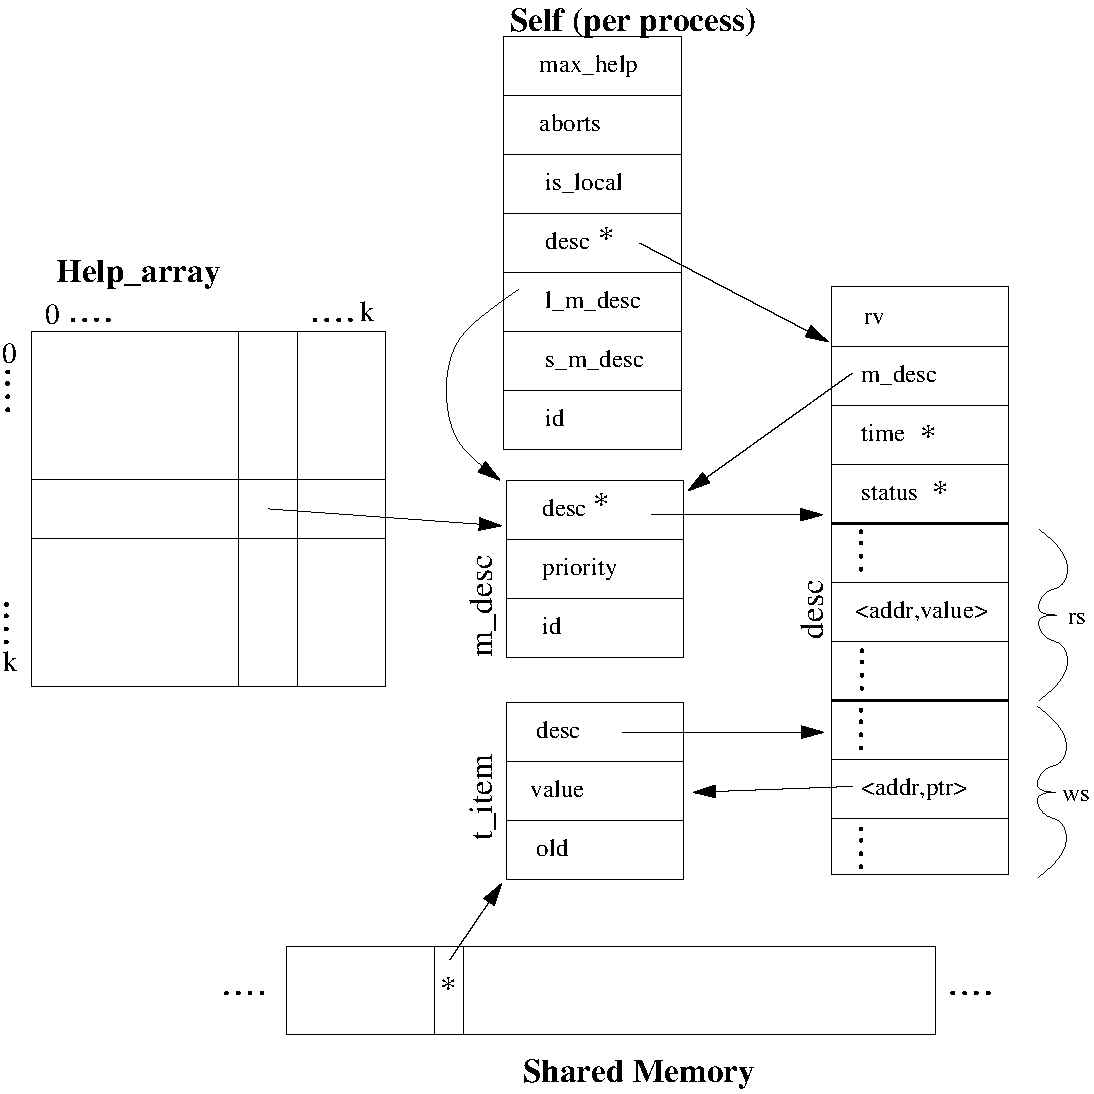
\includegraphics[width=0.9\textwidth]{stuff}}
}
\caption{The memory set-up and the data structures that are used by the 
algorithm.}
\label{fig:mem_setup}
\end{figure*}
 
!!!!!!!!!!!!!!!!!!!!!!!!!! Need to update commit for R/O transactions !!!!!!!!!!!!!!!!!!!
 
\section{Intro}
In \cite{} we presented a universal construction in which every transaction that is started is guaranteed to commit no matter the
concurrecny pattern of the system.
In addition, the progress of each thread was dependent only on the proccessor that it was statically assigned to.
Unfortunatley while this algorithm was realistic in the sense that it could be implemented, it also presented several bottlenecks
for performance.
Of these the two most important are (1) there is a single list containing all transactions, through which every transaction must
traverse to perform reads and validations, before performing a CAS on the head pointer in order to commit, creating a single point
of contention and (2) this list is expensive to maintain both in terms of computation and memory usage.
The goal of the algorithm presented here is to address these bottlenecks.
To acieve this, the idea of having a single list is thrown out for a more traditional view of memory when each variable has its own
unique address.
This memory layout is similar to one that we have used to present an efficent algorithm implementing \emph{terminating strong isolation} \cite{}.
Non-conflicting transactions can then execute concurrently and completely independently (other then accessing a shared clock used for consistency).
A process is still required to help other processes in order to ensure that every transaction is committed, this is done by looking for processes
to help in a shared array where processes announce they need help.



\section{Memory Setup}
Instead of storing values directly at their address in shared memory, this algorithm
uses a level of indirection when a location is read or written to by a transactional read or write.
Each address then stores a pointer to an object of type $t\_item$, which is dereferenced
whenever a transactional read is performed on this location.
Each $\mathit{t\_item}$ contains the following fields:
a pointer $\mathit{desc}$, which points to the descriptor of the transaction $T$ that has written
this value to memory,
the field $\mathit{value}$, which contains the value that $T$ has written,
and the field $\mathit{old}$, containing the value that was previously at this location before
it was updated by $T$.

Every transaction $T$ is made up of two descriptors.
Its main descriptor (an object of type $\mathit{m\_desc\_type}$) which is a unique per transaction, and additional
execution descriptors (object of type $\mathit{desc\_type}$), one per execution of this transaction.
The reason for having separate execution descriptors is that there can be multiple executions of a transaction,
either due to aborts, or due to several threads executing the transaction concurrently in order to help it commit.
The main descrptor contains three fields:
A unique value, $\mathit{priority}$ assigned to the transaction which can be used as a global ordering for all transactions,
$\mathit{id}$, a unique identifier for the process that initialized the transaction, and a pointer $\mathit{desc}$ that points
to an exection descriptor of the transaction.
Each execution descriptor contains the following fields:
$\mathit{rv}$, the value read from the global clock $\mathit{GCV}$ at the start of the transaction,
a pointer, $\mathit{m\_desc}$, to the main descriptor for this transaction,
the unique commit time assocated with this transaction, obtained by performing an ${\sf Increment\&Fetch}$ on the global
clock $\mathit{GCV}$,
an atomic value $\mathit{status}$ describing the current state of this execution of the transaction which a value of either
LIVE meaning the transaction is currently running, COMMITTED meaning this execution of the transaction was successfully committed,
or ABORTED meaning that this execution of the transaction has been aborted,
a set $\mathit{rs}$ of pairs $\tuple{\mathit{addr,value}}$ for each of the locations this transaction has read so far,
and a set $\mathit{ws}$ of pairs $\tuple{\mathit{addr,ptr}}$ for each of the locations this transaction has written to so far, where $\mathit{ptr}$ is 
a pointer to a $\mathit{t\_item}$.

In additon to these structures, a $\mathit{k}$ by $\mathit{k}$ (where $\mathit{k}$ is the number of processes in the system)
array called $\mathit{Help\_array}$ exists in shared memory.
Each location in the array either contains a pointer to a main descriptor to a transaction that needs help or $\bot$.
This array is used for processes to announce to other processes that they need help.
A process with id $\mathit{i}$ will scan the row $\mathit{Help\_array}[\mathit{i}][\mathit{*}]$ when looking for a transaction to help.
When requesting help for a transaction $T$, a process with id $\mathit{i}$ whos execution of $T$ was aborted by process with id $\mathit{j}$, will
annouce that it needs help to process $\mathit{j}$ by setting $\mathit{Help\_array}[\mathit{j}][\mathit{i}]$ to point to the main descriptor of $T$.


\section{Operation description}
Here we have the traditional transactional operations of ${\sf begin\_transaction}$, ${\sf transactional\_read}$, ${\sf transactional\_write}$,
and ${\sf try\_to\_commit}$ from wich the STM system runs.
Within these operations we have calls to other procedures can be grouped into two broad categories (1) the ones that perform simlpe checks such
as validations and (2) the ones that are used to performing the helping of other transactions.
Let us start by examining the simple check type operations show in Figure \ref{fig:helpers}.

\subsection{Small procedures}

\paragraph{get\_value}
Each $t\_item$ stores two possible values for an address,
$\mathit{value}$, which stores the value written by the transaction that created this object,
and $\mathit{old}$, which stores the value written by the last transaction to successfully commit, writing to this locaion.
This procedure simply checks if the transaction that created this item has commited (i.e. $\mathit{item.desc.status}$ = COMMITTED), if
so then $\mathit{value}$ is returned, otherwise $\mathit{old}$ is returned.

\paragraph{validate\_by\_value}
This operation validates the read set of a transaction by value.
It is used during the ${\sf try\_to\_commit}$ operation and simply goes through each location
in the read set, checking if the value currently in memory was the value that was read during the execution of the transaction.
If not then the transaction is aborted by calling ${\sf check\_abort}$ with true as input???

\paragraph{check\_abort}
This procedure takes as input a main descriptor $\mathit{m\_desc}$.
If the transsaction is being executed locally (meaning there cannot be any concurrent processes helping it execute)
then the abort count is increased and transaction is immediately restarted.
Otherwise if the transaction is one that needs help (i.e. is not local) then the ${\sf contention\_manager}$ procedure is called
taking as input the main descriptors of the conflicting transactions.
If this returns false then the transaction is aborted, thus returing back to line \ref{} of the ${\sf help\_loop}$.
If the call to ${\sf contention\_manager}$ returns true then the transaction continues executing (maybe should abort in the case it was called
in validate!!!!!!!!!!!).


\paragraph{contention\_manager}
This procedure takes as input two main descriptors of conflicting transactions, $\mathit{m\_desc}$ is the descriptor of the transaction
that noticed the conflict and $\mathit{o\_m\_desc}$ is the descriptor of the conflicting transaction.
The actions of this operation are based on the priority assigned to the transactions.
If the priority of $\mathit{m\_desc}$ is greater then that of $\mathit{o\_m\_desc}$, then the 


\begin{figure} [htb]
\centering{ \fbox{
\begin{minipage}[t]{1\linewidth}%{150mm}
%\footnotesize 
\scriptsize
\renewcommand{\baselinestretch}{2.5} 
%\resetline
%\setcounter{linecounter}{200}
\begin{tabbing}
aaaaaaa\=aa\=aaaaa\=aa\=aa\=\kill %~\\

{\bf operation} ${\sf get\_value}(\mathit{item})$: \\
\line{H02} \> {\bf if} ($\mathit{item.desc.status}$ = COMMITTED) {\bf then} {\sf return}($\mathit{item.value}$) \\
\line{H02} \>\> {\bf else} {\sf return}($\mathit{item.old}$). \\
{\bf end operation}. \\
\\
{\bf operation} ${\sf validate\_by\_value}()$:\\% {\bf is}\\
% \line{H01} \> $\mathit{rv} \gets \mathit{GVC}$; \\
\line{H02} \> {\bf for each} $\tuple{\mathit{addr, value}}$ in $\mathit{rs}$ {\bf do} \\
\line{H03} \>\> $\mathit{tmp} \gets (\downarrow \mathit{addr})$; \\
\line{H04} \>\> {\bf if} (($\mathit{item} \not \in \mathit{ws} \wedge \mathit{tmp.desc.status} = $ LIVE) $\vee$ (${\sf get\_value}(\mathit{tmp}) \neq \mathit{item.value}$)) \\
% ($\mathit{temp.desc.time} > \mathit{desc.time}$)) \\

!!!!!!!!!!!!!!!!!!!Need to ensure an abort happens here!!!!!!!!!!!!!!!!!!! \\

\line{H05} \>\>\> {\bf then} ${\sf check\_abort}(\mathit{tmp.desc.m\_desc})$; \\
\line{H05} \>\> {\bf end if} \\
\line{H05} \> {\bf end for} \\
{\bf end operation}. \\
\\
{\bf operation} ${\sf check\_abort}(m\_desc)$:\\% {\bf is}\\
\line{AB01} \> {\bf if} ($\mathit{Self.is\_local}$) {\bf then} \\
\line{AB01} \>\> $\mathit{aborts} \gets \mathit{aborts} + 1$; \\
\line{AB02} \>\> the transaction is restarted at ${\sf begin\_transaction}()$ \\
\line{AB01} \> {\bf else if} ($\neg {\sf contention\_manager}(\mathit{Self.s\_m\_desc}, \mathit{m\_desc})$) {\bf then} \\
\line{AB01} \>\> jump back to ${\sf help\_loop}()$ just below the call to ${\sf execute\_transaction}()$;  \\
% \line{AB01} \>\> {\bf end if} \\
\line{AB01} \> {\bf end if} \\
%\line{H21} \> free items in $\mathit{ws}$, $\mathit{rs}$, and $\mathit{ntrs}$; \\
%\line{H22} \> jump to line \ref{START1} \\
{\bf end operation}. \\
\\
{\bf operation} ${\sf contention\_manager}(\mathit{m\_desc}, \mathit{o\_m\_desc})$:\\
\line{AB01} \> {\bf if} ($\mathit{m\_desc.priority} > \mathit{o\_m\_desc.priority}$) \bf{then} \\
\line{AB01} \>\> ${\sf other\_shared\_abort}(\mathit{m\_desc}, \mathit{o\_m\_desc})$; \\
\line{AB01} \>\> {\bf return} ($\sf{true}$); \\
\line{AB01} \> {\bf else if} ($\mathit{m\_desc.priority} = \mathit{o\_m\_desc.priority}$) {\bf then} \\
\line{AB01} \>\> {\bf return} ($\sf{false}$); \\
\line{AB01} \> {\bf else} \\
\line{AB01} \>\> ${\sf self\_shared\_abort}(\mathit{m\_desc}, \mathit{o\_m\_desc})$; \\
\line{AB01} \>\> {\bf return} ($\sf{false}$); \\
\line{AB01} \> {\bf end if}. \\
{\bf end operation}.\\
\\
{\bf operation} ${\sf self\_shared\_abort}(\mathit{m\_desc}, \mathit{o\_m\_desc})$:\\
\line{AB01} \> $\mathit{desc} \gets \mathit{m\_desc.desc}$; \\
\line{AB01} \> $CAS(\mathit{desc.status}, $LIVE$, \mathit{o\_m\_desc.id})$; \\
\line{AB01} \> {\bf if} ($(\mathit{id} \gets \mathit{desc.status}) \neq$ COMMITTED) {\bf then} \\
\line{AB01} \>\> $\mathit{Help\_array}[\mathit{o\_m\_desc.id}][\mathit{Self.id}] \gets m\_desc$; \\
\line{AB01} \> {\bf end if} \\
{\bf end operation}.\\
\\
{\bf operation} ${\sf other\_shared\_abort}(\mathit{m\_desc}, \mathit{o\_m\_desc})$:\\
\line{AB01} \> $\mathit{desc} \gets \mathit{o\_m\_desc.desc}$; \\
\line{AB01} \> $CAS(\mathit{desc.status}, $LIVE$, \mathit{m\_desc.id})$; \\
\line{AB01} \> Need to ask for help? \\
% \line{AB01} \> {\bf if} ($(\mathit{id} \gets \mathit{desc.status.status}) \neq$ COMMITTED) {\bf then} \\
% \line{AB01} \>\> $\mathit{help\_array}[\mathit{o\_m\_desc.id}][\mathit{Self.id}] \gets m\_desc$; \\
% \line{AB01} \> {\bf end if} \\
{\bf end operation}.
\end{tabbing}
\normalsize
\end{minipage}
}
\caption{Transactional helper operations.}
\label{fig:helpers}
}
\end{figure}

 
 
 
 
 \begin{figure} [htb]
\centering{ \fbox{
\begin{minipage}[t]{1\linewidth}%{150mm}
%\footnotesize 
\scriptsize
\renewcommand{\baselinestretch}{2.5} 
%\resetline
%\setcounter{linecounter}{200}
\begin{tabbing}
aaaaaaa\=aa\=aaaaa\=aa\=aa\=\kill %~\\

{\bf operation}  ${\sf begin\_transaction}()$:\\% {\bf is}\\
\line{S1} \> {\bf if} ($\mathit{Self.is\_local}$) {\bf then} \\
\line{S1} \>\> {\bf if} ($\mathit{Self.aborts} = 0$) {\bf then} $\mathit{Self.l\_main\_desc} \gets $ alloc new main descriptor \\
\line{S1} \>\>\> $\mathit{Self.l\_main\_desc.priority} \gets $ unique priority based on $\mathit{GCV}$ and $\mathit{Self.id}$ \\
\line{S1} \>\> {\bf else if} ($\mathit{aborts} > \mathit{THLD}$) {\bf then} \\
% \line{S1} \>\>\> $\mathit{Self.is\_local} \gets \sf{false}$; \\
\line{S1} \>\>\> $\mathit{Help\_array}[\mathit{Self.id}][\mathit{Self.id}] \gets \mathit{Self.l\_main\_desc}$; \\
\line{S1} \>\>\> ${\sf help\_loop}()$; \\
\line{S1} \>\>\> $\mathit{Self.desc} \gets \mathit{Self.l\_main\_desc.desc}$; \\
% \line{S1} \>\>\> $\mathit{Self.is\_local} \gets {\sf true}$; \\
\line{S1} \>\>\> jump to ${\sf try\_to\_commit}()$; \\
\line{S1} \>\> {\bf end if} \\
\line{S1} \> {\bf end if} \\
\line{S1} \> $\mathit{Self.desc} \gets$ allocate new transaction descriptor \\
\line{S1} \> $\mathit{Self.desc.rv} \gets \mathit{GCV}$; \\
{\bf end operation}.\\
\\


{\bf operation} ${\sf try\_to\_commit}()$: \\
\line{S1} \> {\bf if} ($\neg \mathit{Self.is\_local}$) {\bf then} \\
\line{S1} \>\> $\mathit{desc} \gets \mathit{Self.s\_main\_desc.desc}$; \\
\line{S1} \>\> {\bf if} ($\mathit{desc.status.status} =$ ABORTED) {\bf then} \\
\line{S1} \>\>\> $\mathit{desc.time} \gets {\sf GCV}$; \\
% \line{S1} \>\>\> {\bf for each} $(\tuple{\mathit{addr, item}} \in \mathit{ws})$ \\
% \line{S1} \>\>\>\> {\bf do} $\mathit{item.old} \gets {\sf get\_value}(\downarrow \mathit{addr})$; $\mathit{item.time} \gets \mathit{time}$ {\bf end for} \\
\line{S1} \>\>\> $\sf{CAS}(\mathit{Self.s\_main\_desc.desc, desc, Self.desc})$ {\bf end if} \\
\line{S1} \> {\bf else} \\
\line{S1} \>\> {\bf if} (${\sf help\_commit}(Self.desc)$) {\bf then} \\
\line{S1} \>\>\> $\mathit{Self.aborts} \gets 0$; \\
\line{S1} \>\>\> $\sf{help\_loop}()$; \\
\line{S1} \>\>\> {\sf return} ($\sf{true}$). \\
\line{S1} \>\> {\bf end if} \\
\line{S1} \>\> $\mathit{Self.aborts} \gets \mathit{Self.aborts} + 1$; \\
% \line{S1} \>\> {\sf return} ($\sf{false}$). \\
\line{S1} \> {\bf end if} \\
\line{S1} \> {\sf return} ($\sf{false}$). \\
{\bf end operation}.\\
\\
{\bf operation} ${\sf help\_commit}(\mathit{m\_desc})$: \\
\line{E01} \> $\mathit{desc} \gets \mathit{m\_desc.desc}$; $\mathit{status} \gets \mathit{desc.status}$; \\
\line{E01} \> {\bf if} ($\mathit{desc.status} = $ COMMITTED) {\bf then} {\sf return}(${\sf true}$) \\
\line{E01} \> {\bf else if} ($\mathit{desc.status} = $ ABORTED) {\bf then} {\sf return}(${\sf false}$) {\bf end if} \\
\line{E01} \> $\mathit{time} \gets {\sf GCV}$; \\
\line{E01} \> {\bf for each} $(\tuple{\mathit{addr, item}} \in \mathit{ws})$ {\bf do} \\
\line{E01} \>\> $\mathit{tmp} \gets (\downarrow \mathit{addr})$; \\
\line{E01} \>\> {\bf if} ($\mathit{tmp} = \mathit{item}$) {\bf then} ${\sf continue}()$ {\bf end if} \\
\line{E01} \>\> {\bf if} ($\mathit{tmp.desc.status} = $ LIVE) {\bf then} \\
\line{E01} \>\>\> {\bf if} ($\mathit{Self.is\_local}$) {\bf then} {\sf return}(${\sf false}$) {\bf end if} \\
\line{E01} \>\>\> {\bf if} ($\neg {\sf contention\_manager}(\mathit{m\_desc}, \mathit{tmp.desc.m\_desc})$) {\bf then} {\sf return}(${\sf false}$) {\bf end if} \\
\line{E01} \>\> {\bf end if} \\
\line{E01} \>\> {\bf if} ($\mathit{Self.is\_local}$) {\bf then} $\mathit{item.old} \gets {\sf get\_value}(tmp)$; $\mathit{item.desc.time} \gets \mathit{time}$ \\
\line{E01} \>\> {\bf else} \\
\line{E01} \>\>\> {\bf if} (${\sf get\_value}(\mathit{tmp}) \neq \mathit{item.old}$) \\
\line{E01} \>\>\>\> {\bf then} ${\sf self\_shared\_abort}(\mathit{m\_desc}, \mathit{tmp.desc.m\_desc})$; {\sf return}(${\sf false}$) {\bf end if} \\
\line{E01} \>\> {\bf end if} \\
\line{E01} \>\> {\bf if} ($\neg {\sf CAS}(\mathit{addr},\mathit{tmp},\mathit{item})$) \\
\line{E01} \>\>\> {\bf then if} ($(\mathit{tmp} \gets \downarrow \mathit{addr}) \neq \mathit{item}$)  \\
\line{E01} \>\>\>\> {\bf then} ${\sf contention\_manager}(\mathit{m\_desc}, \mathit{tmp.desc.m\_desc})$; {\sf return}(${\sf false}$) {\bf end if} \\
\line{E01} \>\> {\bf end if} \\
\line{E01} \> {\bf end for} \\
\line{E01} \> ${\sf validate\_rs}()$; \\
\line{E01} \> {\bf if} ($\mathit{Self.is\_local}$) {\bf then} $\mathit{desc.time} \gets {\sf Increment\&Fetch}(\mathit{GVC})$ \\
\line{E01} \> {\bf else if} ($(\mathit{time} \gets \mathit{desc.time}) = \infty$) {\bf then} \\
\line{E01} \>\> ${\sf CAS}(\mathit{desc.time},\infty,{\sf Increment\&Fetch}(\mathit{GVC}))$; \\
% \line{E01} \>\> $\mathit{time} \gets \mathit{desc.time}$; \\
\line{E01} \> {\bf end if} \\
% \line{E01} \> {\bf for each} $(\tuple{\mathit{addr, item}} \in \mathit{ws})$ {\bf do} $\mathit{item.time} \gets \mathit{time}$ {\bf end for} \\
\line{E01} \> {\bf if} ($\neg {\sf CAS}(\mathit{desc.status},$LIVE,COMMITTED)) \\
\line{E01} \>\> {\bf then if} ($(\mathit{id} \gets \mathit{desc.status})$) {\bf then} \\
\line{E01} \>\>\>\> {\bf if} ($\neg \mathit{Self.is\_local}$) {\bf then} $\mathit{Help\_array}[\mathit{id}][\mathit{Self.id}] \gets \mathit{m\_desc}$ {\bf end if} \\
\line{E01} \>\>\>\> {\sf return}(${\sf false}$); \\
\line{E01} \>\> {\bf end if} \\
\line{E01} \> {\bf end if} \\
\line{E01} \> {\sf return}(${\sf false}$). \\
% \line{DA12} \> $\mathit{time} \gets {\sf Increment\&Fetch}(\mathit{GVC})$; \\
{\bf end operation}.

\end{tabbing}
\normalsize
\end{minipage}
}
\caption{Transaction begin/commit.}
\label{fig:tbc}
}
\end{figure}
 
 
 
 
 

\begin{figure} [htb]
\centering{ \fbox{
\begin{minipage}[t]{1\linewidth}%{150mm}
%\footnotesize 
\scriptsize
\renewcommand{\baselinestretch}{2.5} 
%\resetline
%\setcounter{linecounter}{200}
\begin{tabbing}
aaaaaaa\=aa\=aaaaa\=aa\=aa\=\kill %~\\


{\bf operation}  ${\sf transactional\_read}(\mathit{addr})$:\\% {\bf is}\\
\line{C01} \> {\bf if} $\mathit{addr} \in \mathit{ws}$  {\bf then} ${\sf return}$ ($\mathit{item.value}$ from $\mathit{addr}$ in $\mathit{ws}$)  {\bf end if} \\
\line{C02} \> $\mathit{tmp} \gets (\downarrow \mathit{addr})$;\\
\line{C03} \> {\bf if} ($\mathit{tmp.desc.status} = $ LIVE $\vee \mathit{item.desc.time} > \mathit{Self.desc.rv}$) \\
\line{C03} \>\> {\bf then} ${\sf check\_abort}(item.desc.m\_desc)$ {\bf end if} \\
\line{C03} \> $\mathit{value} \gets \sf{get\_value}(\mathit{item})$; \\
\line{C03} \> $\mathit{Self.desc.rs} \gets \mathit{Self.desc.rs} \cup \tuple{\mathit{addr},\mathit{value}}$; \\
\line{C03} \> {\sf return} ($\mathit{value}$). \\
{\bf end operation}.\\
\\



{\bf operation}  ${\sf transactional\_write}(\mathit{addr, value})$:\\% {\bf is}\\
\line{D01} \> {\bf if} $\mathit{addr} \not\in \mathit{ws}$  \\
\line{D02} \>\> {\bf then} \> allocate a new variable $item$; \\
\line{D03} \>\>\> $\mathit{item}  \gets (\mathit{(\uparrow Self.desc), value, \bot})$; 
                   $\mathit{Self.desc.ws} \gets \mathit{Self.desc.ws} \cup \tuple{\mathit{addr, item}}$; \\
\line{D04} \>\> {\bf else} \> set $\mathit{item.value}$ with $\mathit{addr}$ in $\mathit{Self.desc.ws}$ to $\mathit{value}$ \\
\line{D05} \> {\bf end if}. \\
{\bf end operation}.
\end{tabbing}
\normalsize
\end{minipage}
}
\caption{Transactional operations for reading and writing a variable.}
\label{fig:tops}
}
\end{figure} 
 
 
 
 
 
\begin{figure} [htb]
\centering{ \fbox{
\begin{minipage}[t]{1\linewidth}%{150mm}
%\footnotesize 
\scriptsize
\renewcommand{\baselinestretch}{2.5} 
%\resetline
%\setcounter{linecounter}{200}
\begin{tabbing}
aaaaaaa\=aa\=aaaaa\=aa\=aa\=\kill %~\\ 

{\bf operation} ${\sf help\_loop}()$: \\
\line{E01} \> $\mathit{Self.is\_local} \gets {\sf false}$; ${\sf init\_help}()$; \\
\line{E01} \> {\bf while} (($\mathit{m\_desc} \gets {\sf find\_next\_help}()$)$\neq \bot$) {\bf do} \\
\line{E01} \>\> $\mathit{desc} \gets \mathit{m\_desc.desc}$; $\mathit{status} \gets \mathit{desc.status}$; \\
\line{E01} \>\> {\bf if} ($\mathit{status} =$ COMMITTED) {\bf then} ${\sf remove\_help}(m\_desc)$ \\
\line{E01} \>\> {\bf else if} ($\mathit{status} =$ LIVE) {\bf then} ${\sf help\_commit}(\mathit{m\_desc})$ \\
\line{E01} \>\> {\bf else} $\mathit{self.s\_main\_desc} \gets \mathit{m\_desc}$; ${\sf execute\_transaction}(m\_desc)$ {\bf end if} \\
\line{E01} \> {\bf end while} \\
\line{E01} \> $\mathit{Self.is\_local} \gets {\sf true}$. \\
{\bf end operation}.\\
\\
{\bf operation} ${\sf init\_help}()$:\\
\line{E01} \> $\mathit{max} \gets 0$; \\
\line{E01} \> {\bf for} ($\mathit{i} = 0; \mathit{i} < \mathit{k}; \mathit{i} \gets \mathit{i} + 1$) {\bf do} \\
\line{E01} \>\> $\mathit{next} \gets \mathit{Help\_array}[\mathit{Self.id}][\mathit{i}]$; \\
\line{E01} \>\> {\bf if} ($\mathit{next} \neq \bot \wedge \mathit{next.desc.status} \neq$ COMMITTED $\wedge \mathit{next.priority} > \mathit{max}$) \\
\line{E01} \>\>\> {\bf then} $\mathit{max} \gets \mathit{next.priority}$ {\bf end if} \\
\line{E01} \> {\bf end for} \\
\line{E01} \> $\mathit{Self.max\_help} \gets \mathit{max}$. \\
{\bf end operation}.\\
\\
{\bf operation} ${\sf find\_next\_help}()$: \\
\line{E01} \> $\mathit{min} \gets \bot$; \\
\line{E01} \> {\bf for} ($\mathit{i} = 0; \mathit{i} < \mathit{k}; \mathit{i} \gets \mathit{i} + 1$) {\bf do} \\
\line{E01} \>\> $\mathit{next} \gets \mathit{Help\_array}[\mathit{Self.id}][\mathit{i}]$; \\
\line{E01} \>\> {\bf if} ($\mathit{next} \neq \bot \wedge \mathit{next.priority} \leq \mathit{Self.max\_help} \wedge \mathit{next.desc.status} \neq$ COMMITTED) \\
\line{E01} \>\>\> {\bf then} $\mathit{min} \gets \mathit{next}$; ${\sf break}()$ {\bf end if} \\
\line{E01} \> {\bf end for} \\
\line{E01} \> {\bf for} ($\mathit{i}; \mathit{i} < \mathit{k}; \mathit{i} \gets \mathit{i} + 1$) {\bf do} \\
\line{E01} \>\> $\mathit{next} \gets \mathit{Help\_array}[\mathit{Self.id}][\mathit{i}]$; \\
\line{E01} \>\> {\bf if} ($\mathit{next} \neq \bot \wedge \mathit{next.desc.status} \neq$ COMMITTED $\wedge \mathit{next.priority} \leq \mathit{min.priority}$) \\
\line{E01} \>\>\> {\bf then} $\mathit{min} \gets \mathit{next}$ {\bf end if} \\
\line{E01} \> {\bf end for} \\
\line{E01} \> {\sf return} ($\mathit{min}$). \\
{\bf end operation}.
\end{tabbing}
\normalsize
\end{minipage}
}
\caption{Helping operations}
\label{fig:hops}
}
\end{figure} 
 
 
 
 
 
\end{document}
 
